\documentclass[twocolumn,a4paper,10pt]{article}

\usepackage[utf8]{inputenc}
\usepackage{t1enc}
\usepackage[spanish]{babel}
\usepackage[pdftex,usenames,dvipsnames]{color}
\usepackage[pdftex]{graphicx}
\usepackage{enumerate}
\usepackage{url}
\usepackage{amsmath}
\usepackage{amsfonts}
\usepackage{amssymb}
\usepackage[table]{xcolor}
\usepackage[small,bf]{caption}
\usepackage{float}
\usepackage{subfig}
\usepackage{bm}
\usepackage{fancyhdr}
\usepackage{times}
\usepackage{titlesec}
\usepackage[numbers]{natbib}
\usepackage{titling}
\usepackage{listings}

\renewcommand{\lstlistingname}{Código Fuente}

%%% Listings
\lstloadlanguages{Octave} 
\lstdefinelanguage{MyOctave}[]{Octave}{% 
	deletekeywords={beta,det},
	morekeywords={repmat}
} 
\lstset{ %
	language=MyOctave,
	stringstyle=\ttfamily,
	showstringspaces = false,
	basicstyle=\footnotesize\ttfamily,
	commentstyle=\color{gray},
	keywordstyle=\bfseries,
	numbers=left,
	numberstyle=\ttfamily\footnotesize,
	stepnumber=1,                   % the step between two line-numbers. If it's 1 each line will be numbered
	framexleftmargin=0.10cm,
	numbersep=0.05cm,               % how far the line-numbers are from the code
	backgroundcolor=\color{white},
	showspaces=false,
	showtabs=false,
% 	frame=l,
	tabsize=4,
	captionpos=b,                   % sets the caption-position to bottom
	breaklines=true,                % sets automatic line breaking
	breakatwhitespace=false,        % sets if automatic breaks should only happen at whitespace
	mathescape=true
}

\def\customabstract{\vspace{.5em}
    {\small\center{\textbf{RESUMEN}} \\[0.5em] \relax%
}}
\def\endkeywords{\par}

\def\keywords{\vspace{.5em}
    {\textit{Palabras clave: } 
}}
\def\endkeywords{\par}

\titleformat{\section}{\small\center\bfseries}{\thesection.}{0.5em}{\normalsize\uppercase}
\titleformat{\subsection}{\small\center\bfseries}{\thesubsection}{0.5em}{\small\uppercase}
\titleformat{\subsubsection}{\small\bfseries}{}{0.5em}{\small}
\renewcommand{\bibsection}{}

% TITLE Configuration
\setlength{\droptitle}{-30pt}
\pretitle{\begin{center}\Huge\begin{rmfamily}}
\posttitle{\par\end{rmfamily}\end{center}\vskip 0.5em}
\preauthor{\begin{center}
        \large \lineskip 0.5em%
\begin{tabular}[t]{c}}
\postauthor{\end{tabular}\normalsize 
    \\[1em] Estudiantes del Instituto Tecnológico de Buenos Aires
\par\end{center}}
\predate{\begin{center}\small}
\postdate{\par\end{center}}

% Headers
\addtolength{\voffset}{-40pt}
\addtolength{\textheight}{80pt}
\renewcommand{\headrulewidth}{0pt}
\fancyhead{}
\fancyfoot{}
\lhead{\small No publicado: Cátedra de Métodos Numéricos Avanzados (ITBA)}
\rhead{\small \thepage}
\cfoot{\small Copyright \copyright 2012 ITBA}

% Metadata
\title{Estudio y simulaci\'on de accidente nuclear}
\date{23 de Noviembre de 2012}
\author{Civile, Juan Pablo \and Crespo, Álvaro \and Ordano, Esteban }

\begin{document}

\pagestyle{fancy}
\maketitle
\thispagestyle{fancy}

\begin{customabstract}
\textbf{
El objetivo del presente trabajo es simular y analizar el comportamiento de los radionucleidos expulsados a la atm\'osfera durante un accidente nuclear, similar al 
de Chernobyl \footnote{El accidente nuclear ocurrido el 26 de april de 1986 en Chernobyl, Ucrania es considero el peor desastre nuclear de la historia \cite{Chernobyl}.}, 
utilizando la \textit{ecuaci\'on de difusi\'on-advecci\'on} y aplicando un esquema expl\'icito centrado para discretizarla.
}
\end{customabstract}

\begin{keywords}
radionucleidos, nube radiactiva,  ecuaci\'on difusi\'on-advecci\'on, discretizaci\'on, delta de Dirac
\end{keywords}

\section{Introducci\'on}

Cuando ocurre un accidente nuclear, los radionucleidos liberados a la atm\'osfera son afectados por 2 procesos: la difusi\'on de los radionucleidos en el aire, y
la advecci\'on por el movimiento la masa de aire debido al viento. Para modelar el proceso de contaminaci\'on atmosf\'erica puede considerarse que la concentraci\'on de
contaminante $u(x,y,z,t)$ satisface la \textit{ecuaci\'on difusi\'on-advecci\'on}

\begin{equation}
\label{ec:difusion-adveccion}
    \frac{\partial u}{\partial t} + \nabla \cdot (y \vec{v}) = k \nabla^2 u
\end{equation}

donde $\vec{v} (x,y,z,t)$ es la velocidad del viento  y k, el coeficiente de difusi\'on de la atm\'osfera. Dicha ecuaci\'on tiene en cuenta tanto el proceso de 
difusi\'on como el de advecci\'on. El objetivo del presente trabajo es resolver num\'ericamente esta ecuaci\'on para estudiar el comportamiento de estos procesos 
para el caso \textit{bidimensional}.\\

En la secci\'on \ref{sec:metodologia} proponemos y explicamos la discretizaci\'on de la ecuaci\'on \ref{ec:difusion-adveccion} utilizando un esquema expl\'icito 
centrado.\\
En la secci\'on \ref{sec:resultados} se muestran los resultados obtenidos, junto con el an\'alisis de cada uno. \\
Finalmente, en la secci\'on \ref{sec:conclusiones} se interpretan los resultados obtenidos y se detallan las conclusiones m\'as importantes. \\

\section{Metodolog\'ia}
\label{sec:metodologia}
Consideramos el caso bimensional, donde $u = u(x,y,t)$ y la ecuaci\'on \ref{ec:difusion-adveccion} se escribe como \cite{Guia2-MNA}

\begin{equation}
\label{ec:difusion-adveccion-2D}
\frac{\partial u}{\partial t} + \frac{\partial (uv_{x})}{\partial x} + \frac{\partial (uv_{y})}{\partial y}  = k \left(\frac{\partial^2 u}{\partial x^2} + \frac{\partial^2 u}{\partial y^2}\right)
\end{equation}

Para nuestro caso de estudio, tomaremos $k = 0,025$ y $v$, la velocidad del viento est\'a dada por 

\begin{equation}
    \vec{v} = v_{0}(\cos (2\pi f_{0}t), \sin (2\pi f_{0}t))
\end{equation}

donde $v_{0} = 2$ y $f_{0} = \frac{1}{3600}$. La fuente puede considerarse casi toda concentrada en una regi\'on muy pequeña, es decir casi una 
delta de Dirac \cite{Guia2-MNA}. Este sería el ``hipocentro'' o \textit{ground-zero} \cite{groun-zero} del desastre. \\

Para la discretizaci\'on del problema, aplicamos un esquema expl\'icito centrado a la ecuaci\'on \ref{ec:difusion-adveccion-2D}, resultando en 

\begin{equation}
\label{ec:discretizacion}
\begin{array}{c}
\dfrac{u_{i,j}^{n+1} - u_{i,j}^{n}}{2\Delta t} + v_{x}\dfrac{u_{i+1,j}^{n} - u_{i-1,j}^{n}}{2\Delta x} +  v_{y}\dfrac{u_{i,j+1}^{n} - u_{i,j-1}^{n}}{2\Delta y} \\
    \\
    = k \left( \dfrac{u_{i+1,j}^{n} - 2u_{i,j}^{n} + u_{i-1,j}^{n}}{\Delta x^2} - \dfrac{u_{i,j+1}^{n} - 2u_{i,j}^{n} + u_{i,j-1}^{n}}{\Delta y^2}  \right)
\end{array}       
\end{equation}

Aqu\'i la notaci\'on utilizada es la siguiente: \\
$u_{i, j}^{n} = u(i\Delta x, j\Delta y, n\Delta t$).
De la ecuaci\'on \ref{ec:discretizacion} se puede despejar $u_{i,j}^{n+1}$, resultando en la ecuaci\'on \ref{ec:discretizacion-despejada}, que permite calcular 
de forma iterativa $u(x,y,t)$ dado el estado inicial $u_{0}$.

\begin{equation}
\label{ec:discretizacion-despejada}
\begin{array}{c}
u_{i,j}^{n+1} = 2\Delta t \left[ k \left( \dfrac{u_{i+1,j}^{n} - 2u_{i,j}^{n} + u_{i-1,j}^{n}}{\Delta x^2} - \dfrac{u_{i,j+1}^{n} - 2u_{i,j}^{n} + u_{i,j-1}^{n}}{\Delta y^2}  \right) \right.\\
     \\
 \left. - v_{x}\dfrac{u_{i+1,j}^{n} - u_{i-1,j}^{n}}{2\Delta x} -  v_{y}\dfrac{u_{i,j+1}^{n} - u_{i,j-1}^{n}}{2\Delta y} \right] + u_{i,j}^{n} \\
    \\
\end{array}       
\end{equation}

\section{Resultados}
\label{sec:resultados}

Los par\'ametros elegidos fueron:

\begin{equation}
    \nonumber
    \begin{array}{c c c}
        \Delta x & = & 0,01 \\
        \Delta y & = & 0,01 \\
        \Delta t & = & 0,0001 \\
    \end{array}
\end{equation}

Para simular el estado inicial en el que la fuente est\'a toda concentrada en un solo punto, asignamos a la configuraci\'on inicial $u_{0}$ una matriz 
cuadrada de ceros de una cierta dimensi\'on (en nuestro caso 50), con la particularidad de que en el centro introducimos un valor de 10000, que simular\'ia
la delta de Dirac. En la figura \ref{fig:inicial} podemos ver este estado inicial.\\

La figura \ref{fig:10-iteraciones} muestra la configuraci\'on luego de 10 iteraciones. Podemos observar como la nube se expande en todas las direcciones, 
manteniendo una alta concentraci\'on. Sigue centrada en su posici\'on inicial pero observamos que su expansi\'on no es sim\'etrica. Este efecto es ocasionado 
por la advecci\'on del viento. \\

En la figura \ref{fig:40-iteraciones} se puede ver la simulaci\'on al t\'ermino de 40 iteraciones. La nube no se encuentra mucho más dispersa pero se 
comienza a apreciar de forma m\'as marcada la anti-simetr\'ia. Y observamos un par de detalles m\'as, la intensidad es mayor en la parte inferior y pareciera
expandirse m\'as hacia abajo. De nuevo, estos efectos pueden atribuirse a la advecci\'on del viento.\\ 

La figura \ref{fig:90-iteraciones} muestra el estado de la simulaci\'on luego de la iteraci\'on 90. Aqu\'i ya la superficie abarcada por la nube es 
considerablemente mayor, y se sigue observando en su centro la mayor concentraci\'on de material radioactivo. Adem\'as ya es apreciable el desplazamiento hacia 
abajo sobre el eje vertical por el efecto del viento.\\

La figura \ref{fig:350-iteraciones} muestra la etapa final de la simulaci\'on: iteraci\'on 350. La superficie de la nube abarca gran parte del 3er cuadrante, 
pero la itensidad ya ha disminuido considerablemente. También se observa un leve desplazamiento hacia la izquierda en el eje horizontal, sumado al ya mencionado 
desplazamiento hacia abajo sobre el vertical. \\

La figura \ref{fig:1000-iteraciones} muestra el final de la simulaci\'on, luego de la iteraci\'on 1000. Ya imagen muestra casi completamente negra, con algunos muy 
pocos puntos con cierta intensidad en el margen inferior izquierdo, casi imperceptibles al ojo humano.


\section{Conclusiones}
\label{sec:conclusiones}

A partir de las simulaciones realizadas podemos concluir que el efecto del viento tiene dos grande efectos sobre la dispersi\'on de material radioactivo. Estos son, 
la deformaci\'on y el desplazamiento de la nube a lo largo del tiempo. Aunque ambos efectos esten presentes durante toda la simulaci\'on, la deformaci\'on se hace
m\'as notoria durante la primera etapa de expansi\'on, durante la cual se aprecia la falta de simetr\'ia en la expansi\'on de la nube. 
Por otro lado, el desplazamiento reci\'en se aprecia en el largo plazo.


\section*{Referencias}

\begin{thebibliography}{99}

    \bibitem{Guia2-MNA} Fierens, Pablo I. Gu\'ia 2 de M\'etodos Num\'ericos Avanzados, Instituto Tecnol\'ogico de Buenos Aires, 2012.
    \bibitem{Chernobyl} \url{http://en.wikipedia.org/wiki/Chernobyl_disaster}
    \bibitem{groun-zero} \url{http://en.wikipedia.org/wiki/Ground_zero}
    
\end{thebibliography}

\clearpage
\section*{Anexo 1: C\'odigo Fuente}

    \lstinputlisting[caption=tp3.m,label=code:dft,mathescape=false]{../src/tp3.m}

\clearpage
\section*{Anexo 2: Im\'agenes}

\begin{figure}[H]
        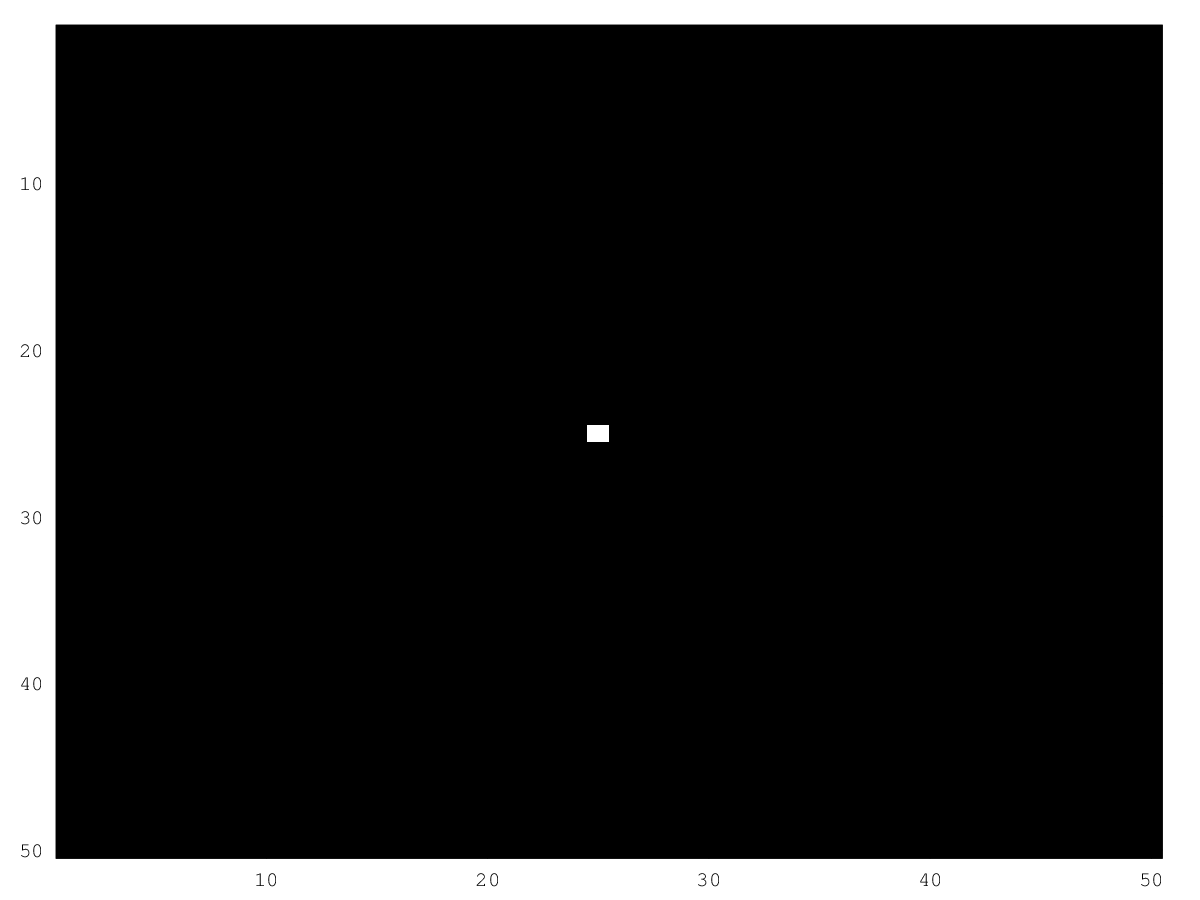
\includegraphics[width=\linewidth]{./images/iteration-1.png}
        \caption{Imagen del estado inicial. Toda la concentraci\'on contaminante esta un solo punto, simulando la delta de Dirac.}
        \label{fig:inicial}
\end{figure}

\begin{figure}[H]
        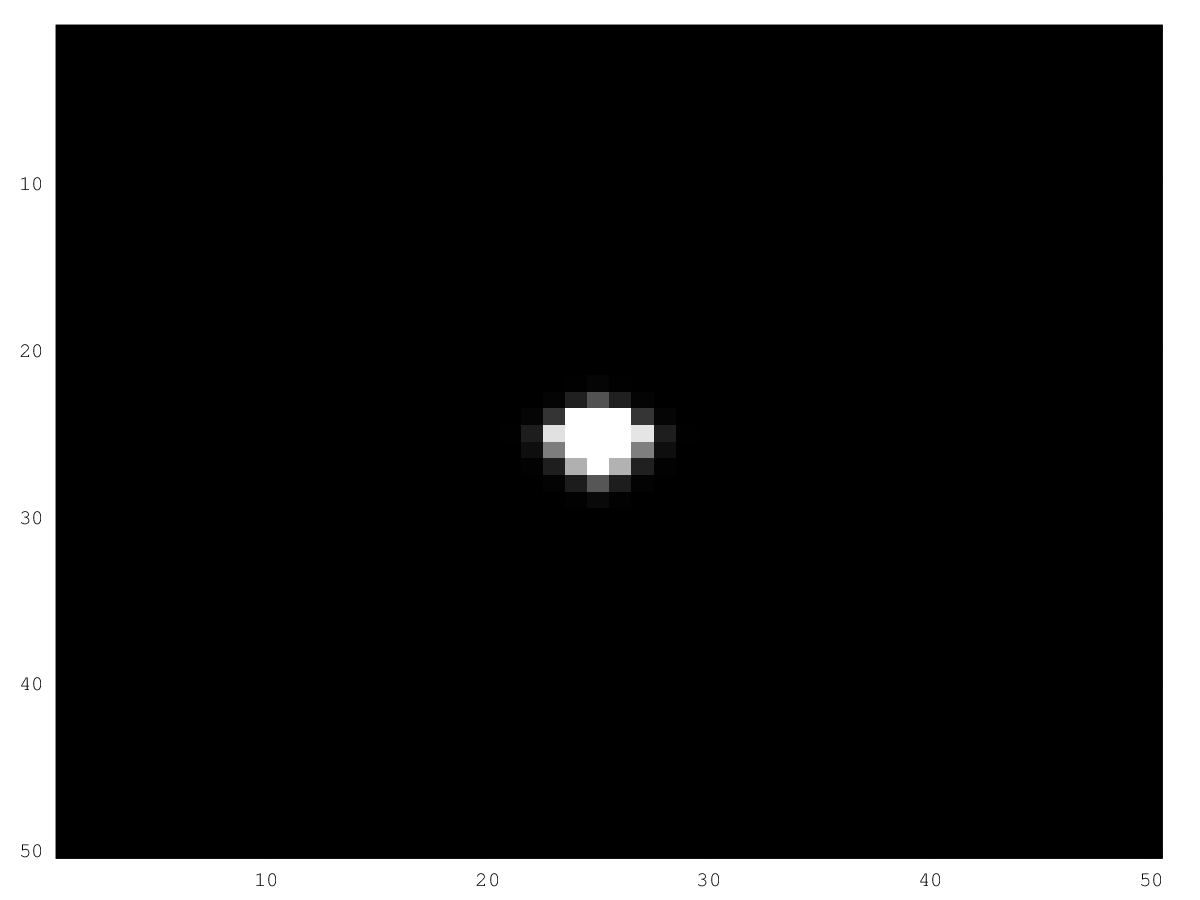
\includegraphics[width=\linewidth]{./images/iteration-10.png}
        \caption{Imagen de la etapa inicial de la simulaci\'on: iteraci\'on 10. La nube comienza a expandirse. Se puede observar que no lo hace de maner sim\'etrica. 
        Esto es causado por la advecci\'on del viento.}
        \label{fig:10-iteraciones}
\end{figure}

\begin{figure}[H]
        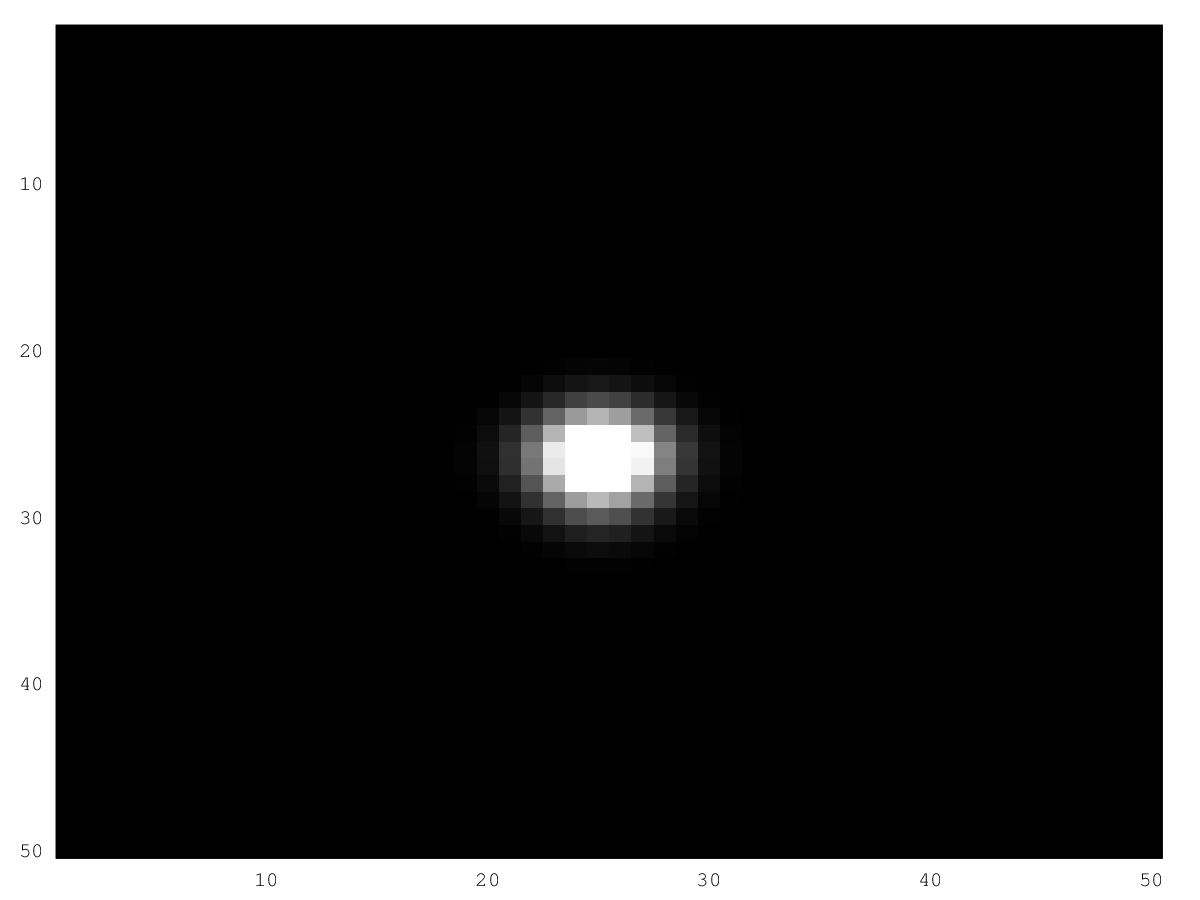
\includegraphics[width=\linewidth]{./images/iteration-40.png}
        \caption{Imagen de la iteraci\'on 40. Se observan 2 efectos m\'as causados por el viento, la mayor concentraci\'on de en la parte inferior de la nube, y 
        la mayor expansi\'on hacia abajo.}
        \label{fig:40-iteraciones}
\end{figure}

\begin{figure}[H]
        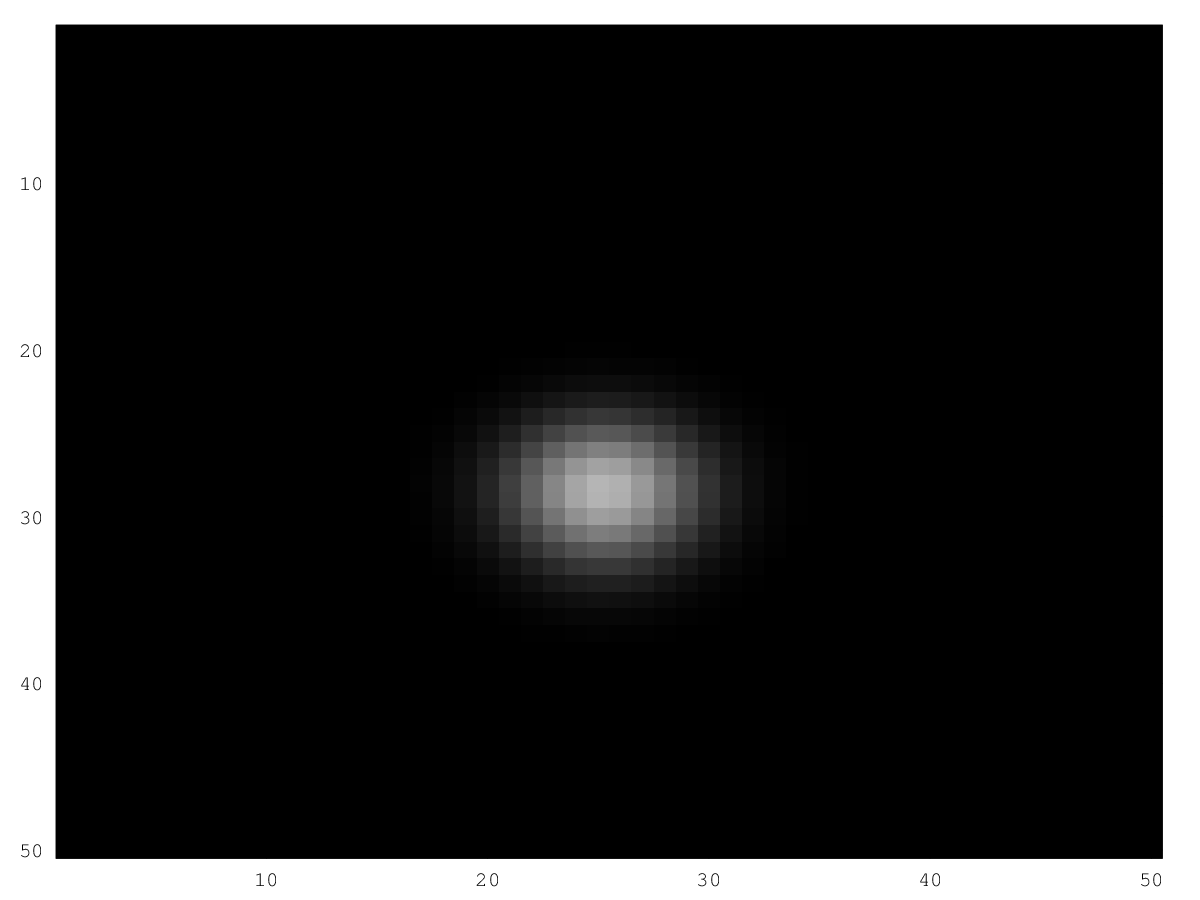
\includegraphics[width=\linewidth]{./images/iteration-90.png}
        \caption{Imagen de la itraci\'on 90 de la simulaci\'on. La superficie abarcada por la nube es considerablemente mayor y además se puede observar 
        el desplazamiento hacia abajo en el eje vertical.}
        \label{fig:90-iteraciones}
\end{figure}

\begin{figure}[H]
        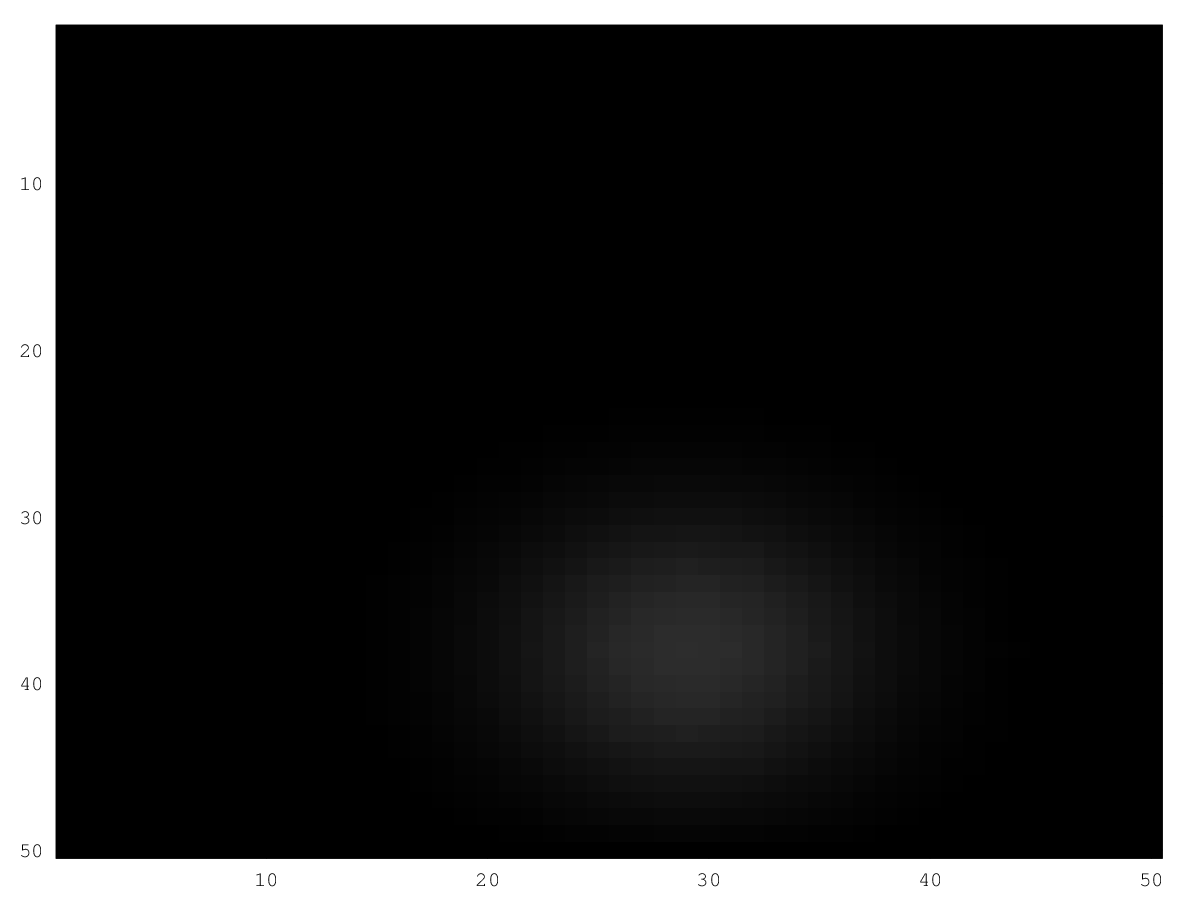
\includegraphics[width=\linewidth]{./images/iteration-350.png}
        \caption{Imagen de la itraci\'on 350 de la simulaci\'on. Etapa final de la simulaci\'on, la nube ya est\'a bien dispersa y su concentraci\'on ha 
        disminuido considerablemente. Adem\'as se observa un leve desplazamiento hacia la izquierda en el eje horizontal.}
        \label{fig:350-iteraciones}
\end{figure}

\begin{figure}[H]
        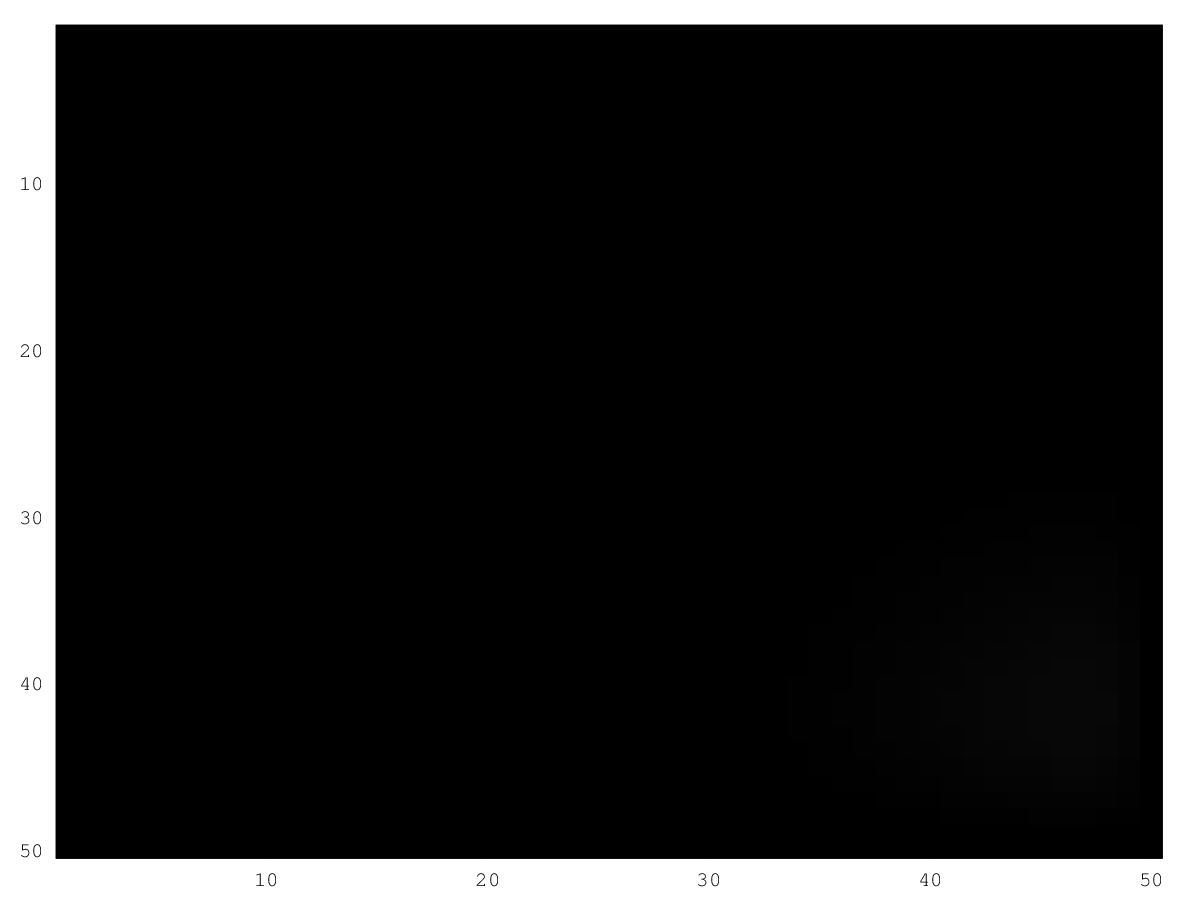
\includegraphics[width=\linewidth]{./images/iteration-1000.png}
        \caption{Imagen de la itraci\'on 1000 de la simulaci\'on. Fin de la simulaci\'on. La nube ya es casi imperceptible. Existen ciertos puntos en el margen 
        inferior izquierdo de la imagen con cierto concentraci\'on. Esto muestra que toma m\'as de 1000 iteraciones en dispersarse completamente la nube radiactiva.}
        \label{fig:1000-iteraciones}
\end{figure}

\end{document}
